\documentclass[12 pt, a4paper]{article}
\usepackage[norsk]{babel}  								% For norsk oppsett
\usepackage[utf8]{inputenc}
\usepackage{amsmath}
\usepackage{amssymb}
\usepackage{graphicx}
\usepackage{subcaption}
\usepackage{hyperref}
\usepackage{fancyhdr}
\usepackage{enumerate}
\usepackage{float}
\usepackage{tikz}
\usepackage{circuitikz}
\usepackage{physics}
\usepackage[includeheadfoot, margin =1cm]{geometry}
%\usepackage{python}
\usepackage[version=3]{mhchem}
\usepackage{siunitx}
\usepackage{todonotes}
\usepackage{xcolor}
\usepackage{lastpage}
\usepackage{listings}
\renewcommand{\exp}[1]{\mathrm{e}^{#1}}

\lstset{basicstyle=\ttfamily,
  showstringspaces=false,
  commentstyle=\color{red},
  keywordstyle=\color{blue}
}

\usepackage[bottom]{footmisc}
\renewcommand\footnoterule{\rule{\linewidth}{0.5pt}}

\setlength{\parindent}{0cm}

\author{Erik Skaar\\ erikfsk@uio.no}





\begin{document}
\pagebreak


\pagestyle{fancy}
\fancyhf{}
\rhead{MEK1100}
\lhead{Erik Skaar}
\fancyfoot[CE,LO]{\leftmark}
\fancyfoot[LE,RO]{Page \number\value{page} of \pageref{LastPage}}

\renewcommand{\headrulewidth}{2pt}
\renewcommand{\footrulewidth}{1pt}

\subsection*{1 a)}

\textbf{Finn tiden $t_m$ når ballen faller ned på bakken ($y=0$) og
posisjonen $x(t_m) = x_m$ hvor dette skjer.}
\\
\\
Vi får oppgitt at:
\begin{align*}
    &x(t) = v_0t \cos{\theta}
    \\
    &y(t) = v_0t \sin{\theta} - \frac{1}{2}gt^2
\end{align*}

Vi vet at $t_m$ er når ballen treffer bakken. Det er når $y(t) = 0$.
Vi løser ligningen over for dette tilfellet:

\begin{align*}
    &y(t) = v_0t \sin{\theta} - \frac{1}{2}gt^2
    \\
    &0 = v_0t_m \sin{\theta} - \frac{1}{2}gt_m^2
    \\
    &v_0t_m \sin{\theta} = \frac{1}{2}gt_m^2
    \\
    &t_m = 2 \frac{v_0}{g}\sin{\theta}
\end{align*}

For å finne $x_m$ bruker vi $t_m$ i formelen for x(t):

\begin{align*}
    &x(t) = v_0t \cos{\theta}
    \\
    &x_m = v_0t_m \cos{\theta}
    \\
    &x_m = 2 \frac{v_0^2}{g}\sin{\theta} \cos{\theta}
\end{align*}


\subsection*{1 b)}

\textbf{Innfør dimensjonsløse variable $(x^*,y^*,t^*)$ for x,y,t når du skalerer
 med $x_m$ for lengde og $t_m$ for tid. Forklar hvorfor det ikke er behov for å
 skalere vinkelen $\theta$.}
\\
\\
Vi skalerer x og y med $x_m$ og t med $t_m$. Det gir:

\begin{align*}
    t^* = \frac{t}{t_m}
    \qquad
    x^* = \frac{x}{x_m}
    \qquad
    y^* = \frac{y}{x_m}
\end{align*}

% For $y_m$ velger jeg å skalere med toppunktet til $y(t)$.
% Det finner vi ved å sette inn en halv $t_m$ (fordi dette er en parabel
% og toppunktet halvveis mellom to ekvivalente verdier):
%
% \begin{align*}
%     &y(t) = v_0t \sin{\theta} - \frac{1}{2}gt^2
%     \\
%     &y(0.5t_m) = v_0\frac{v_0}{g}\sin{\theta} \sin{\theta}
%     - \frac{1}{2}g\frac{v_0^2}{g^2}\sin^2{\theta}
%     \\
%     &y(0.5t_m) = \frac{v_0^2}{g}\sin^2{\theta}
%     - \frac{1}{2}\frac{v_0^2}{g}\sin^2{\theta}
%     \\
%     &y(0.5t_m) = \frac{1}{2}\frac{v_0^2}{g}\sin^2{\theta}
% \end{align*}
%
% Dermed blir den dimensjonsløse variabelen for y:
%
% \begin{align*}
%     y^* = y/y(0.5t_m)
% \end{align*}


\pagebreak
\subsection*{1 c)}

\textbf{Bruk Matlab eller Python for å tegne abner ($x^*$,$y^*$) for tre
utkastvinkler $\theta_n$ for n = 1,2,3. Velg $0<\theta_1 < \frac{\pi}{4}$,
$\theta_2 = \frac{\pi}{4}$ og $\frac{\pi}{4} < \theta_3 < \frac{\pi}{2}$.
Tegn de tre banene i samme koordinatsystem, og angi hvilken bane som svarer
til hvilken utkastvinkel. Forklar hvorfor disse diagrammene kan brukes til
å finne ballens baner for forskjellige verdier av utgangsfart $v_0$ og
forskjellige verdier av g.}


\begin{figure}[H]
		\centering
		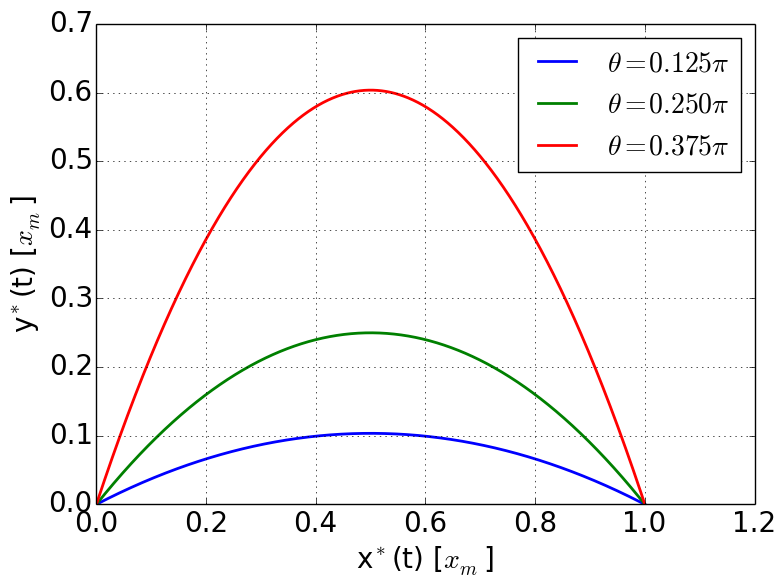
\includegraphics[width=0.7\linewidth]{../1a.png}
		\caption{Grafen viser hvordan banene til ballene med forskjellige
        utkastvinkel vil være i xy-planet. Programmet som ble brukt for
        å lage denne figuren finner du bakerst i innleveringen.}
		\label{fig_a1}
\end{figure}

Disse diagrammene kan brukes til å finne ballens baner for forskjellige verdier
av utgangsfart $v_0$ og forskjellige verdier av g. Trikset er at informasjonen
er lagret i aksene. Altså for at en skal kunne se på effekten av g og $v_0$, må en
pakke ut informasjonen fra aksene. De dimensjonsløse variablene gjør at
alle verdier for g og $v_0$ med samme utkastvinkel gir samme kurve.

\pagebreak
\subsection*{2 a)}
\textbf{Finn strømlinjene.}
\\
\\
Vi har fått oppgitt hastighetsfeltet:

\begin{align*}
    \textbf{v} = v_x\textbf{i} + v_y \textbf{j} =  xy\textbf{i} + y \textbf{j}
\end{align*}

Det er også gitt hint om at denne kan være separabel og vi vet fra
GF at $v_x \dd x = v_y \dd y$ er en nyttig relasjon for å finne strømlinjene:

\begin{align*}
    v_x \dd y &= v_y \dd x
    \\
    xy \dd y &= y\dd x
    \\
    x\dd y &= 1\dd x
    \\
    \int 1 \dd y &= \int \frac{1}{x} \dd x
    \\
    y &= \log(x) + C_0
    \\
    y - \log(x) &= C
\end{align*}















\pagebreak
\subsection*{2 b)}

\textbf{Tegn strømlinjene \sout{for hånd} og sett på piler
for å indikere retningen på strømmen. Et stagnasjonspunkt er et
punkt hvor hastighetsfeltet er lik null. Finn alle stagnasjonspunktene
og identifiser hvor i plottet disse ligger. Det er vanlig å tegne
individuelle stagnasjonspunkter som tjukke kulepunkter.
\\
\\
Vis også at du får til å tegne strømlinjene ved hjelp av
\sout{Matlab eller} Python. Dette kan kanskje vise seg å være en utfordring nær x = 0.}

\begin{figure}[H]
		\centering
		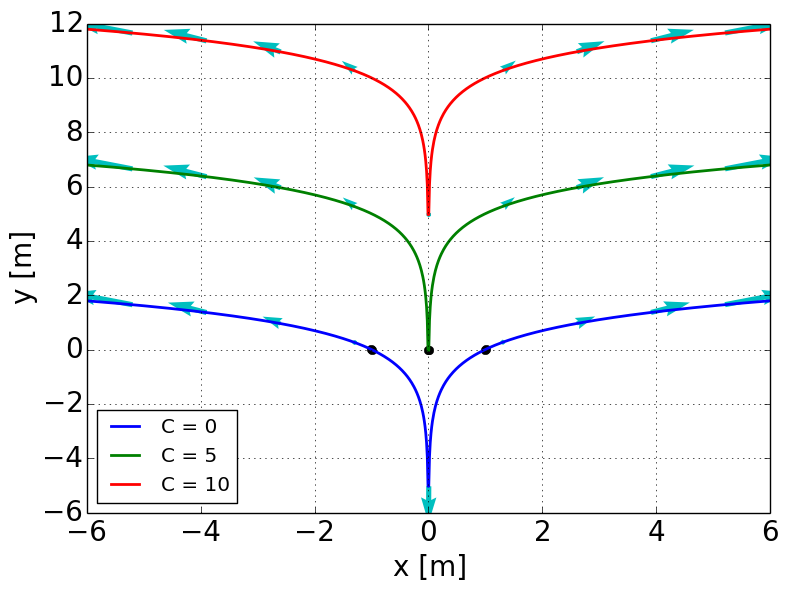
\includegraphics[width=0.7\linewidth]{../2b.png}
		\caption{Figuren viser tre kurver med forskjellige $C$.
        På kurvene er strømvektorene vist som lyseblå vektorer
         og stagnasjonspunkter er vist som svarte prikker.}
		\label{fig_2b_test}
\end{figure}

Figur \ref{fig_2b_test} viser strømlinjene til hastighetsfeltet som
ble oppgitt i oppgave 2. Langs strømlinjene er strømvektorene også
tegnet. Retningen til strømvektorene er tangentiell til strømlinjene.
Det er uendelig mange stagnasjonspunkter langs x-aksen, hvor to og to hører
til en C-verdi.
\\
\\
Jeg glemte å tegne for hånd.








\pagebreak
\subsection*{2 c)}
\textbf{Vis at det ikke finnes en strømfunksjon $\psi$.}
\\
\\
Det blir gitt hint om at det er to måter å vise at feltet ikke har en
strøm funksjon. Regn ut strømfunksjonen og vis at det er en selvmotsigelse
eller hvis at divergensen er ulik null.
\\
\\
Vi skal selvfølgelig gjøre begge:
\\
\\
\\
\begin{align*}
    &v_x = -\partial \psi / \partial y
    && v_y = \partial \psi / \partial x
    \\
    &\psi = -\int v_x \dd y
    &&\psi = \int v_y \dd x
    \\
    &\psi = -\int xy \dd y
    &&\psi = \int y \dd x
    \\
    &\psi = - \frac{1}{2} xy^2
    &&\psi =  xy
\end{align*}

Dette er en åpenbar selvmotsigelse. $\psi$ kan ikke være så bipolar at den
er $xy$ og $- \frac{1}{2} xy^2$ samtidig.
\\
\\
\\
\\

Divergensen er lik $\nabla \cdot \textbf{v} = \partial v_x /\partial x
+  \partial v_y /\partial y$. Med hastighetsfeltet vårt gir det:

\begin{align*}
    \frac{\partial v_x}{\partial x}
    +
    \frac{\partial v_y}{\partial y}
    &=
    \frac{\partial xy}{\partial x}
    +
    \frac{\partial y}{\partial y}
    \\
    \\
    \frac{\partial xy}{\partial x}
    =
    y
    &\qquad \qquad
    \frac{\partial y}{\partial y}
    =
    1
    \\
    \\
    \nabla \cdot \textbf{v} &= \underline{\underline{y + 1 \neq 0}}
    \\
    \\
\end{align*}






%

\pagebreak
\subsection*{3 a)}
\textbf{Finn divergensen $\nabla \cdot \textbf{v} = \partial v_x /\partial x
+  \partial v_y /\partial y$ og virvlingen $\nabla \cross \textbf{v} =
\left(\partial v_y /\partial x - \partial v_x /\partial y\right)\textbf{k}$
av hastighetsfeltet.}
\\
\\
Vi får oppgitt:

\begin{align*}
    v_x = \cos(x)\sin(y), \qquad v_y = - \sin(x)\cos(y)
    \\
\end{align*}

Det gir at divergensen, $\nabla \cdot \textbf{v} = \partial v_x /\partial x
+  \partial v_y /\partial y$, er lik:

\begin{align*}
    \frac{\partial v_x}{\partial x}
    +
    \frac{\partial v_y}{\partial y}
    &=
    \frac{\partial \cos(x)\sin(y)}{\partial x}
    +
    \frac{\partial - \sin(x)\cos(y)}{\partial y}
    \\
    \\
    \frac{\partial \cos(x)\sin(y)}{\partial x}
    =
     -\sin(x)\sin(y)
    &\qquad \qquad
    \frac{\partial - \sin(x)\cos(y)}{\partial y}
    =
    \sin(x)\sin(y)
    \\
    \\
    \nabla \cdot \textbf{v} &= \sin(x)\sin(y) - \sin(x)\sin(y)
    = \underline{\underline{0}}
    \\
    \\
\end{align*}

Videre kan vi finne virvlingen, $\nabla \cross \textbf{v} =
(\partial v_y /\partial x+  \partial v_x /\partial y) \textbf{k}$:


\begin{align*}
    \left(\frac{\partial v_y}{\partial x}
    -
    \frac{\partial v_x}{\partial y}\right) \textbf{k}
    &=
    \left(\frac{\partial -\sin(x)\cos(y)}{\partial x}
    -
    \frac{\partial \cos(x)\sin(y)}{\partial y}\right) \textbf{k}
    \\
    \\
    \frac{\partial - \sin(x)\cos(y)}{\partial x}
    =
     -\cos(x)\cos(y)
    &\qquad \qquad
    \frac{\partial \cos(x)\sin(y)}{\partial y}
    =
    \cos(x) \cos(y)
    \\
    \\
    \nabla \cross \textbf{v}
    &=
    -\cos(x)\cos(y) - \cos(x)\cos(y)\textbf{k}
    =
    \underline{\underline{-2\cos(x)\cos(y)\textbf{k}}}
\end{align*}










\pagebreak
\subsection*{3 b)}
\textbf{Tegn opp strømvektorer langs x- og y-aksen.}
\\
\\
\begin{figure}[H]
		\centering
		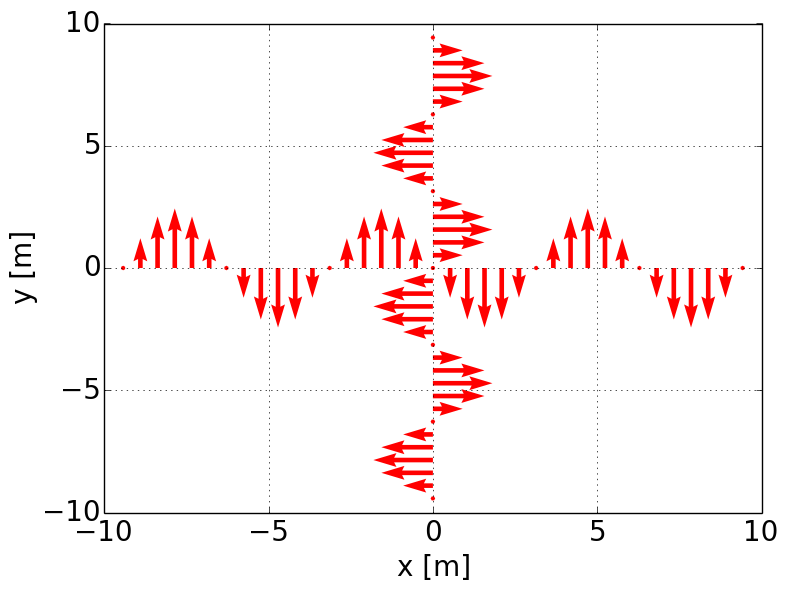
\includegraphics[width=0.7\linewidth]{../3b.png}
		\caption{Vektorene viser hvordan strømvektorene
        er langs x- og y-aksen. Dette er en sin-funksjon langs aksene.}
		\label{fig_3b}
\end{figure}



For å sjekke om figur \ref{fig_3b} er korrekt kan en se generelt
på hastighetsfeltet langs x-aksen og y-aksen:


\begin{align*}
    &\textbf{Langs x-aksen er $ y = 0$}
    &&\textbf{Langs y-aksen er $ x = 0$}
    \\
    &v_x = \cos(x)\sin(y) = 0
    &&v_x = \cos(x)\sin(y) = \sin(y)
    \\
    &v_y = - \sin(x)\cos(y) = -\sin(y)
    &&v_y = - \sin(x)\cos(y) = 0
\end{align*}

Dermed vet vi at vi burde få piler langs aksene som varierer
som en sin-kurve i størrelse.










\pagebreak
\subsection*{3 c)}

\textbf{Finn sirkulasjonen om randa til kvadratet
definert ved $-\frac{\pi}{2} \leq x \leq \frac{\pi}{2}$ og
$-\frac{\pi}{2} \leq y \leq \frac{\pi}{2}$.}
\\
\\
Vi vet fra GF at sirkulasjonen er definert som linjeintegralet
 over hastighetsfeltet. Vi deler opp integralet i 4 deler. En del for
 hver sideflate (starter ved nedre sideflate og beveger oss mot klokken):

\begin{align*}
    C =  \oint \mathbf{v} \dd r
    =
    \int_{a}^{b} \mathbf{v} \cdot \dd \mathbf{r}
    +
    \int_{b}^{c} \mathbf{v} \cdot \dd \mathbf{r}
    +
    \int_{c}^{d} \mathbf{v} \cdot \dd \mathbf{r}
    +
    \int_{d}^{a} \mathbf{v} \cdot \dd \mathbf{r}
\end{align*}

For a til b er $\dd \mathbf{r} = \dd x \mathbf{i}$.
For b til c er $\dd \mathbf{r} = \dd y \mathbf{j}$.
For c til d er $\dd \mathbf{r} = \dd x \mathbf{-i}$.
For d til a er $\dd \mathbf{r} = \dd y \mathbf{-j}$.
Dette gir oss følgende integraler og resultater:

\begin{align*}
    &\int_{a}^{b} \mathbf{v} \cdot \dd \mathbf{r}
    =
    \int_{-\frac{\pi}{2}}^{\frac{\pi}{2}}
    \mathbf{v} \cdot \dd x \mathbf{i}
    =
    \int_{-\frac{\pi}{2}}^{\frac{\pi}{2}}
    \cos(x)\sin(y) \dd x
    = 2 sin(y)
    \\
    &\int_{b}^{c} \mathbf{v} \cdot \dd \mathbf{r}
    =
    \int_{-\frac{\pi}{2}}^{\frac{\pi}{2}}
    \mathbf{v} \cdot \dd y \mathbf{j}
    =
    \int_{-\frac{\pi}{2}}^{\frac{\pi}{2}}
    - \sin(x)\cos(y) \dd y
    = -2\sin(x)
    \\
    &\int_{c}^{d} \mathbf{v} \cdot \dd \mathbf{r}
    =
    \int_{-\frac{\pi}{2}}^{\frac{\pi}{2}}
    \mathbf{v} \cdot \dd x \mathbf{-i}
    =
    \int_{-\frac{\pi}{2}}^{\frac{\pi}{2}}
    -\cos(x)\sin(y) \dd x
    = -2 \sin(y)
    \\
    &\int_{d}^{a} \mathbf{v} \cdot \dd \mathbf{r}
    =
    \int_{-\frac{\pi}{2}}^{\frac{\pi}{2}}
    \mathbf{v} \cdot \dd y \mathbf{-j}
    =
    \int_{-\frac{\pi}{2}}^{\frac{\pi}{2}}
    \sin(x)\cos(y) \dd y
    = 2 \sin(x)
    \\
    &\oint \mathbf{v} \dd r
    =
    2\sin(\frac{\pi}{2})
    + 2\sin(\frac{-\pi}{2})
    - 2\sin(\frac{\pi}{2})
    - 2\sin(\frac{-\pi}{2}) = -8
\end{align*}

 % Ved hjelp av Greens teorem får vi at
 % linje integralet er ekvivalent med flatearealet over virvlingen:

 % \begin{align*}
 %    C =  \oint \mathbf{v} \dd r
 %    =\int_{-\frac{\pi}{2}}^{\frac{\pi}{2}}
 %    \int_{-\frac{\pi}{2}}^{\frac{\pi}{2}}
 %    -2\cos(x)\cos(y)\textbf{k} \cdot \textbf{n} \mathbf{k}
 %    \qquad \dd x \dd y = 0
 % \end{align*}














\subsection*{3 d)}
\textbf{Forklar hvorfor det eksisterer en strømfunksjon for
feltet gitt i likning (1), se hintet i forrige oppgave.
 Vis at strømfunksjonen kan skrives }

 \begin{align}
    \psi = cos(x)cos(y)
 \end{align}

I hintene fra forrige oppgave står det at dersom et vektorfelt
er todimensjonalt i xy-planet, $\mathbf{v} = v_x \mathbf{i}
+ v_y \mathbf{j}$ og divergensfritt, $\partial v_x /\partial x
+  \partial v_y /\partial y = 0$, så eksisterer det en
 strømfunksjon som angitt ovenfor.
\\
\\
Ovenfor får vi definisjonen $v_x = \partial \psi /\partial y$
og $v_y = \partial \psi /\partial x$. Dermed er det bare å integre $v_x$
med hensyn på y og $v_y$ med hensyn på x.


\begin{align*}
    \int v_y \dd x
    &= \int - \sin(x)\cos(y) \dd x
    = \underline{\underline{\cos(x)\cos(y)}}
    \\
    - \int v_y \dd x
    &= - \int \cos(x)\sin(y) \dd x
    = \underline{\underline{\cos(x)\cos(y)}}
\end{align*}




















\pagebreak
\subsection*{3 e)}

\textbf{Bruk Taylorutvikling av andre orden til å
 finne tilnærmede strømlinjer nær origo.}


\begin{align*}
    &\psi(x,y) = T_2(\psi) + \mathcal{O}(x^3,y^3)
\end{align*}

Vi er kun interessert i $T_2(\psi)$ rundt origo:

\begin{align*}
    T_2(\psi)_{0,0} =
    &\psi(0,0)
    +
    \left(\frac{\partial \psi}{\partial x}\right)_{0,0} (x-0)
    +
    \left(\frac{\partial \psi}{\partial y}\right)_{0,0} (y-0)
    +
    \\
    &\frac{1}{2}
    \left(\frac{\partial^2 \psi}{\partial x^2}\right)_{0,0} (x-0)^2
    +
    \frac{1}{2}
    \left(\frac{\partial^2 \psi}{\partial y^2}\right)_{0,0} (y-0)^2
    +
    \left(\frac{\partial^2 \psi}{\partial x\partial y}\right)_{0,0} (x-0)(y-0)
    \\
    T_2(\psi)_{0,0} =
    &\cos(0)\cos(0)
    -\sin(0)\cos(0)x
    -\cos(0)\sin(0)y
    \\
    &-\frac{1}{2}
    \cos(0)\cos(0)x^2
    -
    \frac{1}{2}
    \cos(0)\cos(0)y^2
    +
    \sin(0)\sin(0)x^2
    \\
    \\
    T_2(\psi)_{0,0} =
    &\underline{\underline{
    1
    -\frac{1}{2}
    x^2
    -
    \frac{1}{2}
    y^2
    }}
\end{align*}





















%

\pagebreak
\subsection*{4 a)}
\textbf{Bruk funksjonen streamfun i et skript,\sout{strlin.m eller} strlin.py,
 som plotter konturlinjer for $\psi$ når $n = 5 \land n =30$.}
 \footnote{$\land$ er kul, men feil å bruke i denne sammenhengen.}

\begin{figure}[H]
    \centering
    \begin{subfigure}{0.3\textwidth}
        \centering
        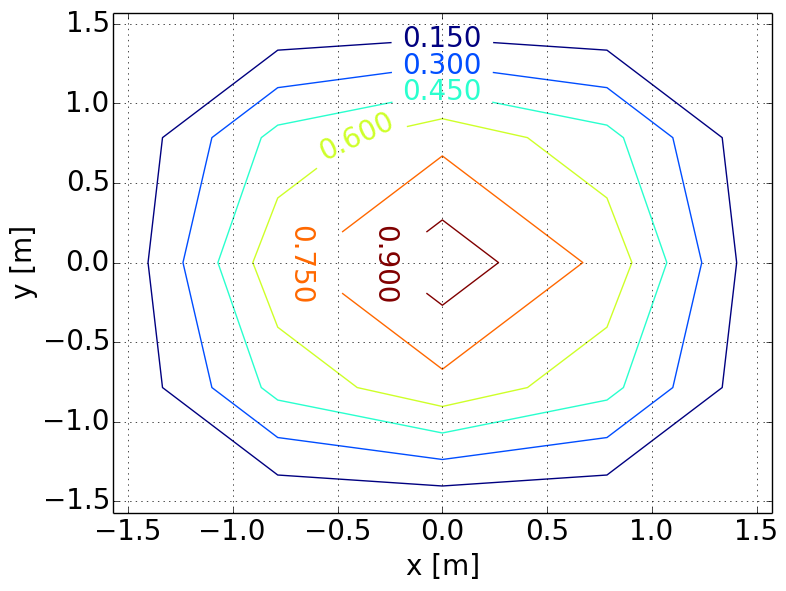
\includegraphics[width=\linewidth]{../4a_0_0,5_5.png}
        \caption{}
    \end{subfigure}%
    ~
    \begin{subfigure}{0.3\textwidth}
        \centering
        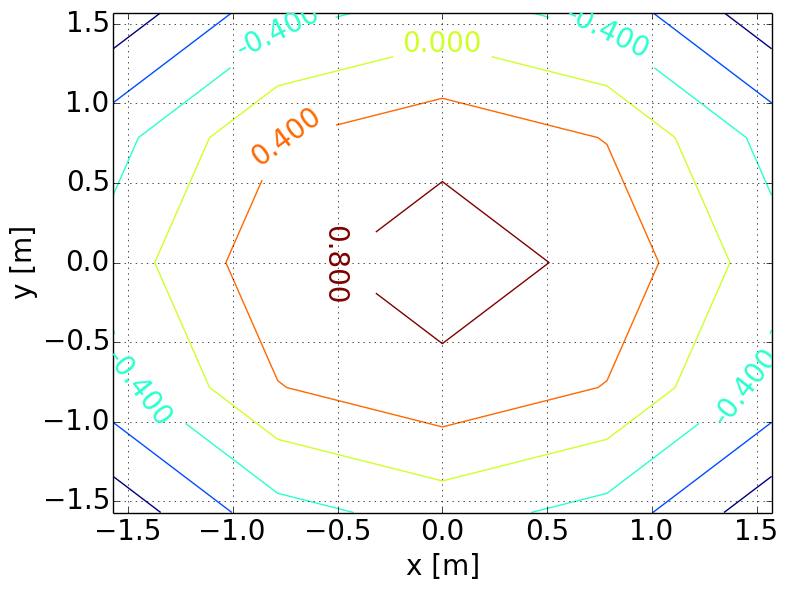
\includegraphics[width=\linewidth]{../4a_1_0,5_5.png}
        \caption{}
    \end{subfigure}
    ~
    \begin{subfigure}{0.3\textwidth}
        \centering
        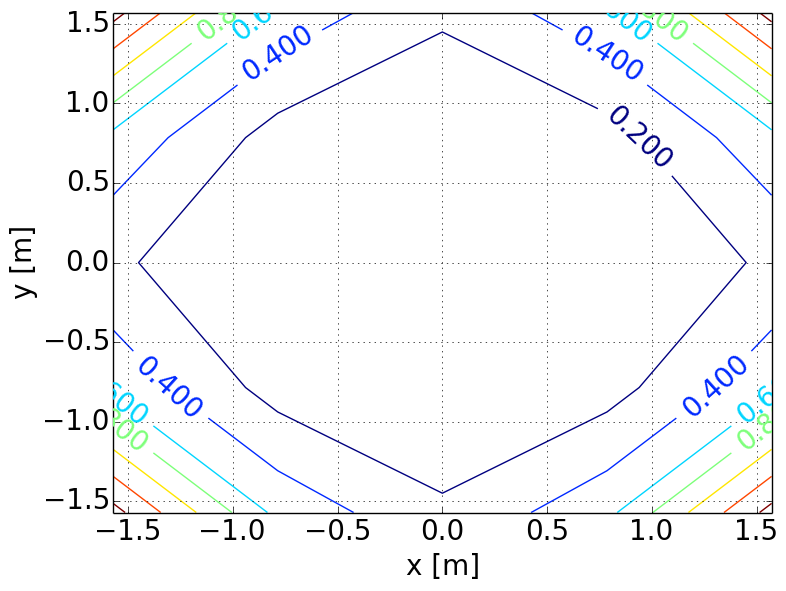
\includegraphics[width=\linewidth]{../4a_2_0,5_5.png}
        \caption{}
    \end{subfigure}
    \caption{Figurene viser $|x| < \frac{\pi}{2}$ og
    $|y| < \frac{\pi}{2}$ med $n = 5$.
    \color{blue} a) \color{black}
     viser konturlinjene
    til $\psi$.
    \color{blue} b) \color{black}
     viser konturlinjene til Taylor approksimasjon
    fra 3 e).
    \color{blue} c) \color{black}
     viser konturlinjene til forskjellen mellom a) og b). }
    \label{fig_4a_first}
\end{figure}

\begin{figure}[H]
    \centering
    \begin{subfigure}{0.3\textwidth}
        \centering
        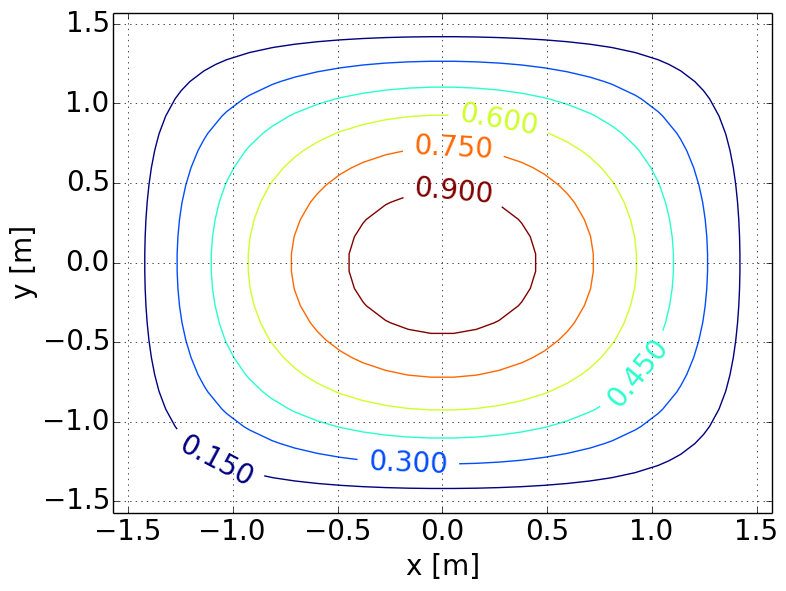
\includegraphics[width=\linewidth]{../4a_0_0,5_30.png}
        \caption{}
    \end{subfigure}%
    ~
    \begin{subfigure}{0.3\textwidth}
        \centering
        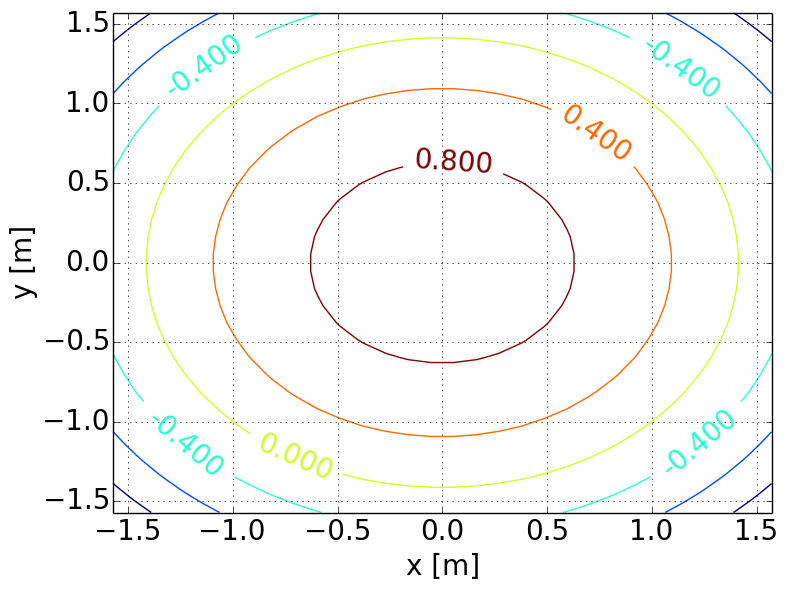
\includegraphics[width=\linewidth]{../4a_1_0,5_30.png}
        \caption{}
    \end{subfigure}
    ~
    \begin{subfigure}{0.3\textwidth}
        \centering
        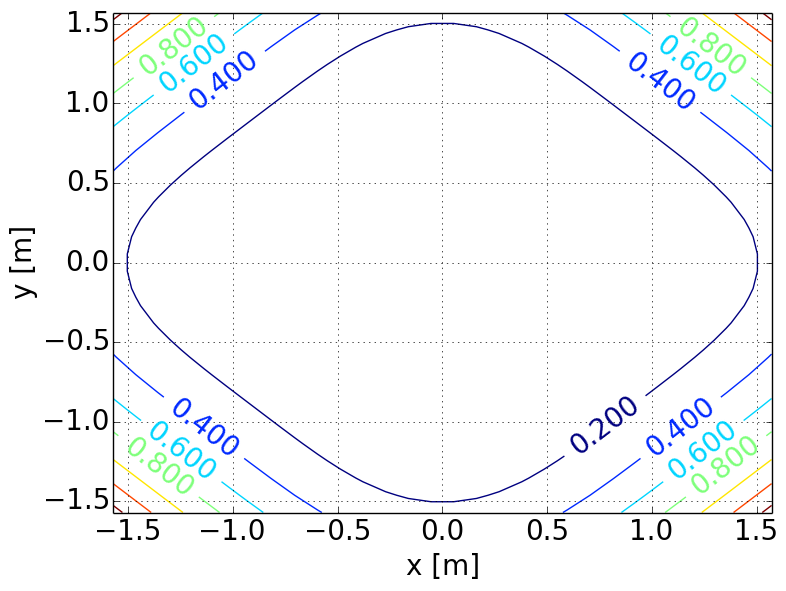
\includegraphics[width=\linewidth]{../4a_2_0,5_30.png}
        \caption{}
    \end{subfigure}
    \caption{Figurene viser $|x| < \frac{\pi}{2}$ og
    $|y| < \frac{\pi}{2}$ med $n = 30$.
    \color{blue} a) \color{black}
     viser konturlinjene
    til $\psi$.
    \color{blue} b) \color{black}
     viser konturlinjene til Taylor approksimasjon
    fra 3 e).
    \color{blue} c) \color{black}
     viser konturlinjene til forskjellen mellom a) og b).}
    \label{fig_4a_second}
\end{figure}

\pagebreak
\begin{figure}[H]
    \centering
    \begin{subfigure}{0.3\textwidth}
        \centering
        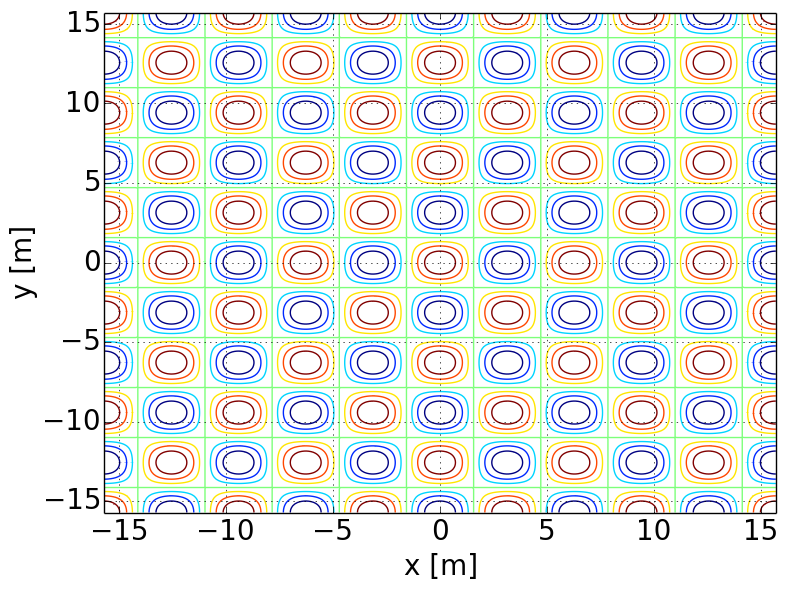
\includegraphics[width=\linewidth]{../4a_0_5_300.png}
        \caption{}
    \end{subfigure}%
    ~
    \begin{subfigure}{0.3\textwidth}
        \centering
        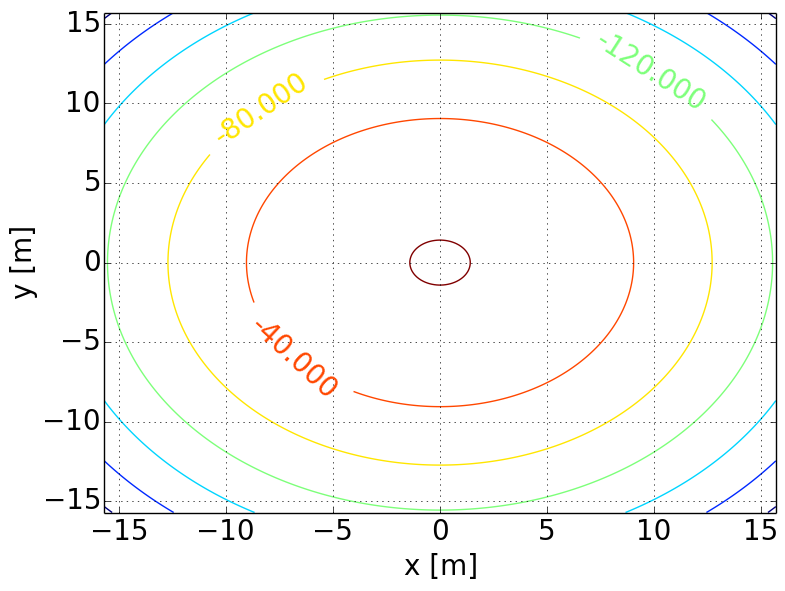
\includegraphics[width=\linewidth]{../4a_1_5_300.png}
        \caption{}
    \end{subfigure}
    ~
    \begin{subfigure}{0.3\textwidth}
        \centering
        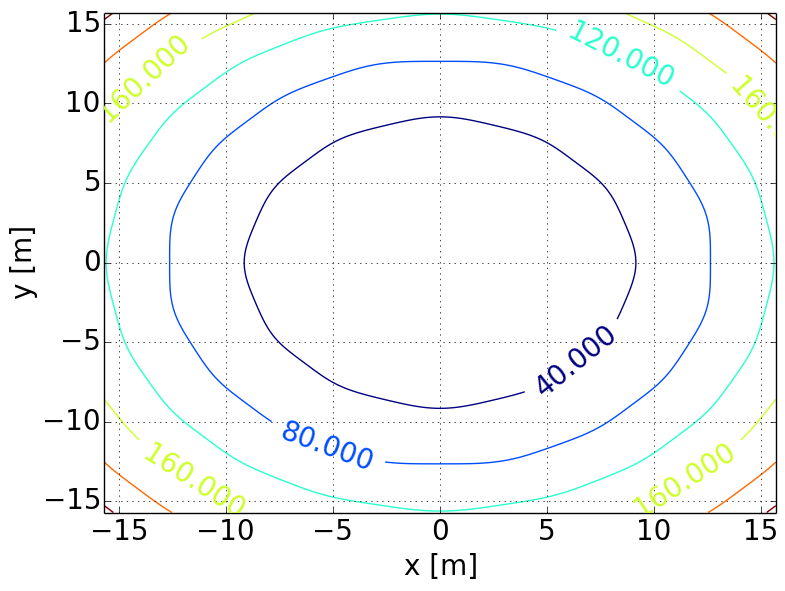
\includegraphics[width=\linewidth]{../4a_2_5_300.png}
        \caption{}
    \end{subfigure}
    \caption{Figurene viser $|x| < \frac{\pi}{2}$ og
    $|y| < \frac{\pi}{2}$ med $n = 30$. \color{blue} a) \color{black}
     viser konturlinjene til $\psi$. \color{blue} b)\color{black} viser
     konturlinjene til Taylor approksimasjon
    fra 3 e). \color{blue} c) \color{black} viser konturlinjene til forskjellen mellom a) og b).}
    \label{fig_4a_third}
\end{figure}

Vi ser at for den første svigningen i $\psi$ approksimasjonen fra
3 e) er ganske god. I figur \ref{fig_4a_first} og figur \ref{fig_4a_second}
vi kan se at det er kun en feil på sirka 0.2 når vi har
kommet til $\frac{\pi}{2}$ på aksene. Dette er å
forvente Taylor approksimasjonen skal være best nærmt
punktet tilnærmingen er laget. Selv om det ikke er blitt spurt om tar
jeg med et plott som viser verdiene til $\psi$ opp til $ 5 \pi $ på aksene
med n satt til 300. I figur \ref{fig_4a_third} kan vi se resultatet.
Jeg tar med dette, fordi det viser hvordan approksimasjonen kun er god rundt
toppen i origo, mens den er helt forferdelig på å tilnærme de andre toppene/bunnene.













\subsection*{4 b)}

\textbf{Skriv en funksjon (\sout{velfield.m eller} velfield.py) som
bergener hastigheter utfra likning (1) ved kallet $x,y,u,v = velfield(n)$.
\\
\\
Bruk denne i et skript, \sout{vec.m eller} vec.py, som tegner et vektorplott
av hastighetsfeltet. Legg vekt på å vlege et passende antall punkter for
lesbarheten av plottet.}

\begin{figure}[H]
    \centering
    \begin{subfigure}{0.5\textwidth}
        \centering
        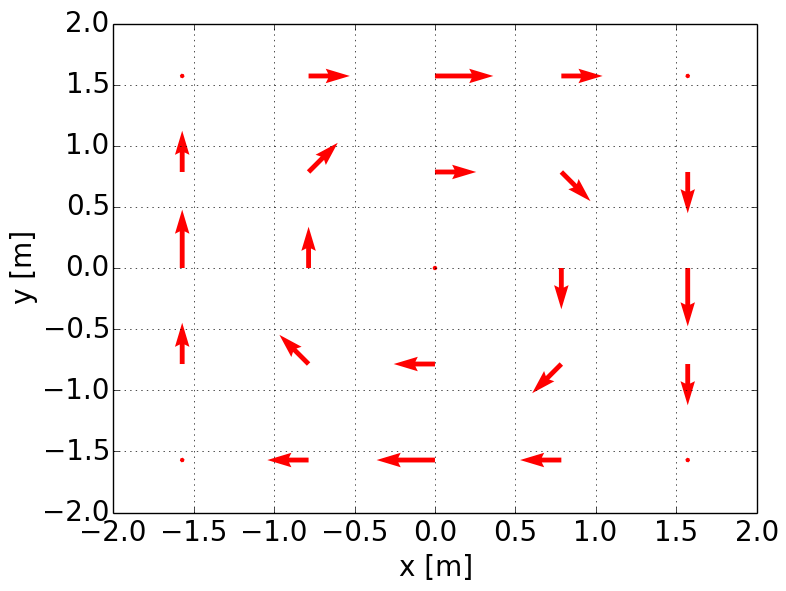
\includegraphics[width=\linewidth]{../4b5.png}
        \caption{}
    \end{subfigure}%
    ~
    \begin{subfigure}{0.5\textwidth}
        \centering
        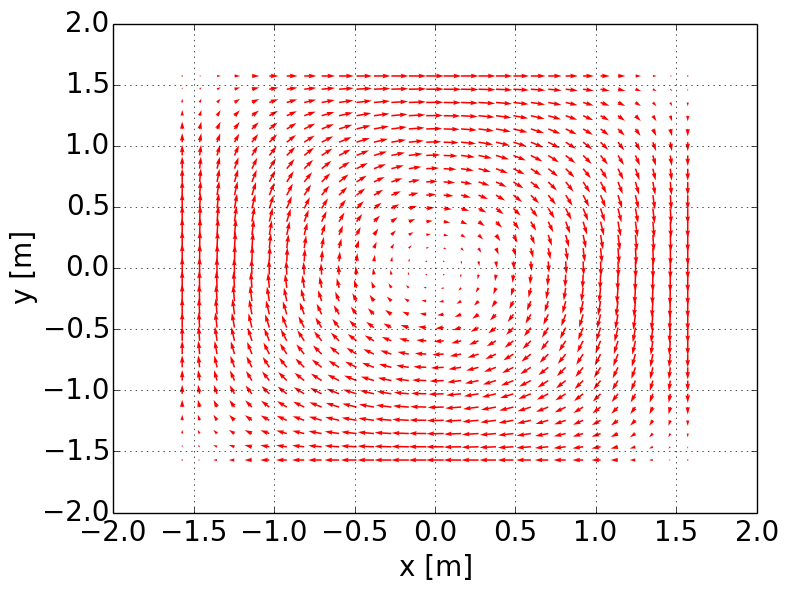
\includegraphics[width=\linewidth]{../4b30.png}
        \caption{}
    \end{subfigure}
    \caption{Figurene viser vektorplott av hastighetsfeltet
    ved hjelp av funksjonen definert i velfield.py. a) er vektorplottet med $n = 5$.
    b) er vektorplottet $n = 30$. }
    \label{fig_4b}
\end{figure}

Figur \ref{fig_4b} er laget ved scriptene beskrevet i oppgaveteksten.
Personlig liker jeg bedre figurer med mange piler (ser mer avansert ut), men
jeg legger ved to varianter slik at det er mer lesbart. 

\pagebreak
\lstinputlisting[language=Python]{../assignment_c1.py}
\pagebreak

\section*{BONUS til oppgave 1b \& c:}
For $y^*$ kan jeg velge å skalere med toppunktet til $y(t)$.
Det finner vi ved å sette inn en halv $t_m$ (fordi dette er en parabel
og toppunktet halvveis mellom to ekvivalente verdier, altså $t = 0$ og $t_m$):

\begin{align*}
    &y(t) = v_0t \sin{\theta} - \frac{1}{2}gt^2
    \\
    &y(0.5t_m) = v_0\frac{v_0}{g}\sin{\theta} \sin{\theta}
    - \frac{1}{2}g\frac{v_0^2}{g^2}\sin^2{\theta}
    \\
    &y(0.5t_m) = \frac{v_0^2}{g}\sin^2{\theta}
    - \frac{1}{2}\frac{v_0^2}{g}\sin^2{\theta}
    \\
    &y(0.5t_m) = \frac{1}{2}\frac{v_0^2}{g}\sin^2{\theta}
\end{align*}

Dermed blir den dimensjonsløse variabelen for y:

\begin{align*}
    y^* = y/y(0.5t_m)
\end{align*}

\begin{figure}[H]
		\centering
		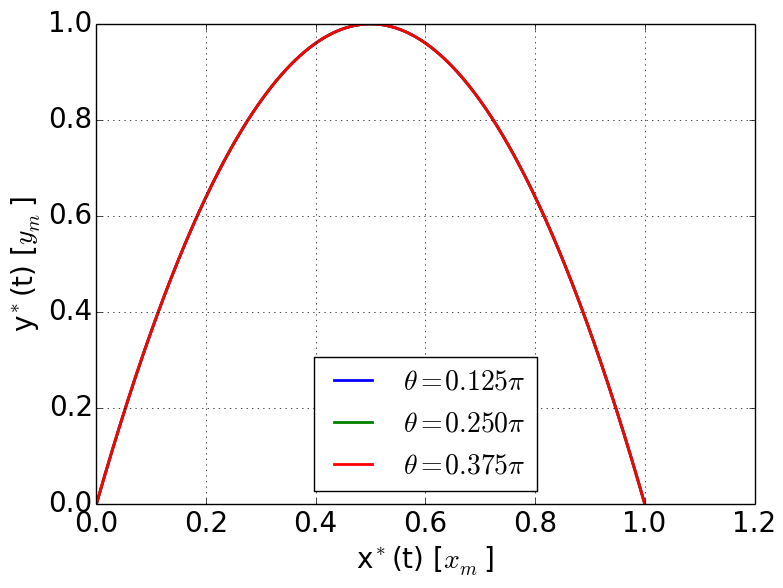
\includegraphics[width=0.7\linewidth]{../alternativ_skalering.png}
		\caption{Grafen viser hvordan banene til ballene med forskjellige
        utkastvinkel vil være i xy-planet. Programmet som ble brukt for
        å lage denne figuren finner du bakerst i innleveringen.}
		\label{fig_alternativ}
\end{figure}

Denne innføringen av dimensjonsløse variabler, gjør at alle kast ser like ut.
Det er en vis sannhet i det (de uttrykkes ved samme formel). Skaleringen gjør
at informasjonen om vinkelen også er pakket inn i aksene, som beskrevet i 1 c).
\pagebreak

\begin{figure}[H]
		\centering
		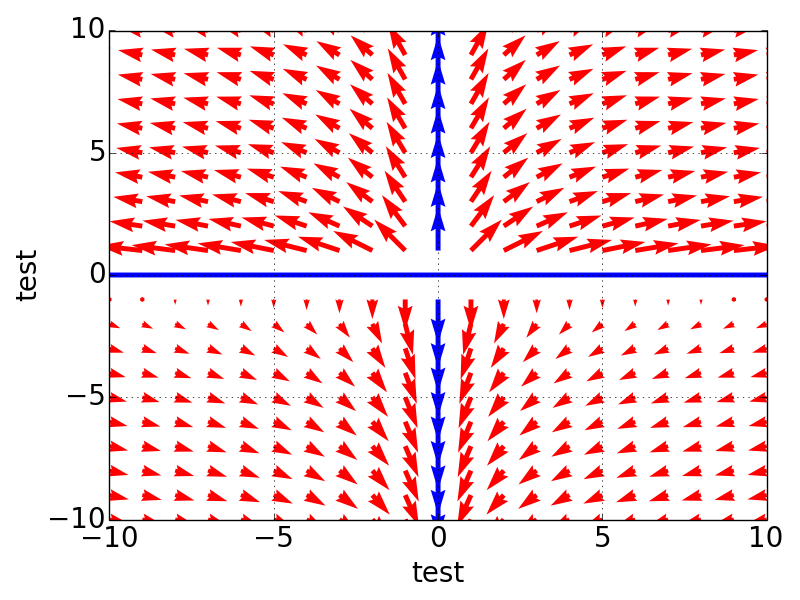
\includegraphics[width=0.7\linewidth]{../test.png}
		\caption{Dette er et tidligere forsøk på å vise
         strømvektorene til 2 b). Fargene er for å gjenskape vårt
         fantastiske flag :).}
		\label{fig_2b_test}
\end{figure}

\pagebreak


\pagebreak
\lstinputlisting[language=Python]{../assignment_b2.py}
\pagebreak
\lstinputlisting[language=Python]{../assignment_b3.py}
\pagebreak

\lstinputlisting[language=Python]{../streamfun.py}
\lstinputlisting[language=Python]{../strlin.py}

\pagebreak
\lstinputlisting[language=Python]{../velfield.py}
\lstinputlisting[language=Python]{../vec.py}


















%



%\begin{align*}
%&n \qquad &2^n - (-1)^n\\
%&n+1 \qquad &2^{n+1} - (-1)^{n+1} \\
%& &= 2(2^{n}) - (-1)^{n+1}\\
%& &= 2(2^{n} + (-1)^n  + (-1)^{n+1}) - (-1)^{n+1}\\
%& &= 2(2^{n} + (-1)^n  - (-1)^{n}) - (-1)^{n+1}\\
%& &= 2(2^{n}- (-1)^{n}) + 2(-1)^n  + (-1)^{n}\\
%& &= 2(2^{n}- (-1)^{n}) + 3(-1)^n \\
%\end{align*}



% \begin{figure}[H]
%     \centering
%     \begin{subfigure}{0.5\textwidth}
%         \centering
%         \includegraphics[width=\linewidth]{result/bilder/Tc/e-Tc}
%         \caption{}
%     \end{subfigure}%
%     ~
%     \begin{subfigure}{0.5\textwidth}
%         \centering
%         \includegraphics[width=\linewidth]{result/bilder/Tc/m-Tc}
%         \caption{}
%     \end{subfigure}
%     \caption{a) Shows how E behaves around $T_C$ b) Shows how |M| develops near $T_C$.}
%     \label{fig:tc-E-M}
% \end{figure}






% \begin{center}
% \label{tab:states-2x2-summary}
% \captionof{table}{The table shows a summary from table \ref{tab:states-2x2}. }
% \begin{tabularx}{\textwidth}{c X c X c X c}
%     \hline
%     \hline
%         Number of $\color{red}{\uparrow}$ && Multiplicity && Energy && Magnetic moment \\
%     \hline
%         4   &&      1      &&      -8J     &&       4       \\
%         3   &&      4      &&      0J      &&       2       \\
%         2   &&      2      &&      8J      &&       0       \\
%         2   &&      4      &&      0J      &&       0       \\
%         1   &&      4      &&      0J      &&       -2      \\
%         0   &&      1      &&      -8J     &&       -4      \\
%     \hline
% \end{tabularx}
% \end{center}













%\begin{tabular}{|c|c|c|c|c|c|c|}
%	\hline
%	n & General & Specific & LU & fastest & slowest & $\frac{slowest}{fastest}$\\
%	\hline
%	10 & 6.5e-05 & 5e-06 & 4e-05 & Specific & General & 13.0\\
%	\hline
%	100 & 7.5e-05 & 8e-06 & 0.0023 & Specific & LU & 287.5\\
%	\hline
%	1000 & 0.00014 & 4e-05 & 0.26 & Specific & LU & 6500\\
%	\hline
%	10000 & 0.0007 & 0.0005 & 142.5 & Specific & LU & 285000 \\
%	\hline
%\end{tabular}







%\begin{figure}[H]
%		\centering
%		\includegraphics[width=0.7\linewidth]{ab.png}
%		\caption{Atomene er gule kuler, de elementære vektorene er blå og a vektorene er grønne.}
%		\label{fig:ab}
%\end{figure}



%\begin{figure}[H]
%		\centering
%		\includegraphics[width=0.7\linewidth]{ab.png}
%		\caption{Atomene er gule kuler, de elementære vektorene er blå og a vektorene er grønne.}
%		\label{fig:ab}
%\end{figure}
%\printbibliography






%\begin{figure}[H]
%    \centering
%    \begin{subfigure}{0.5\textwidth}
%        \centering
%        \includegraphics[width=\linewidth]{maybe}
%        \caption{}
%    \end{subfigure}%
%    ~
%    \begin{subfigure}{0.5\textwidth}
%        \centering
%        \includegraphics[width=\linewidth]{maybe2}
%        \caption{}
%    \end{subfigure}%
%    \caption{a) is probably wrong and b) is right? If not i am not sure what to comment. No matter what. I am not sure what to comment. Cause b) should be wrong. The code above produces a). Setting kb to 1 gives b)}
%\end{figure}








%\begin{align*}
%	J (x,y)=
%	\begin{bmatrix}
%		12x^2 & 1\\
%		1 & 2
%	\end{bmatrix}
%\end{align*}



\end{document}
